%=========================================================================
% Start of
%=========================================================================
\preClass{Graphs of Trigonometric Functions}

\begin{problem}
\item Make a sketch of the sine function.

  \hspace*{-3em}
  \begin{tikzpicture}[y=2cm, x=1.2cm,font=\sffamily]
      % bounds
      \def\lowX{0.0}
      \pgfmathtruncatemacro\startX{round(0.5+\lowX)}
      \pgfmathsetmacro\nextXValue{int(\startX+1)}
      \def\highX{12}
      \def\lowY{-1.25}
      \def\highY{1.25}
      \pgfmathsetmacro\nextYValue{int(\lowY+1)}
      % ticks
      \draw[step = 1, gray, very thin,dashed,opacity=0.85] (0, \lowY) grid ( \highX,\highY);
      % axis
      \draw[thick,->] (0,0) -- coordinate (x axis mid) (\highX,0) node[anchor = south west] {$\theta$};
      \draw[thick,->] (0,\lowY) -- coordinate (y axis mid) (0,\highY) node[rotate=90,yshift=30,anchor = north east] {Sine};

      \draw (1pt, 1) -- (-1pt, 1) node[yshift=-6,xshift=-1,anchor=east] { 1};
      \draw (1pt,-1) -- (-1pt,-1) node[yshift=-6,xshift=-1,anchor=east] {-1};

      \draw (1,1pt) -- (1,-1pt) node[yshift=-1,xshift=0,anchor=north east] {$\frac{ \pi}{2}$};
      \foreach \x in {3,5,...,\highX} {
        \draw (\x,1pt) -- (\x,-1pt) node[yshift=-8,xshift=1,anchor=east] {$\frac{\x\pi}{2}$};
      }
      \draw (2,1pt) -- (2,-1pt) node[yshift=-1,xshift=-1,anchor=north east] {$\pi$};
      \foreach \x in {2,3,...,6} {
        \draw (2*\x,1pt) -- (2*\x,-1pt) node[yshift=-7,xshift=3,anchor=east] {$\x\pi$};
      }
      \draw (6,1.3) node [anchor=south] {The Sine Function};
    \end{tikzpicture}

\item Make a sketch of the sine function shifted left $\frac{\pi}{2}$ units.

  \hspace*{-3em}
  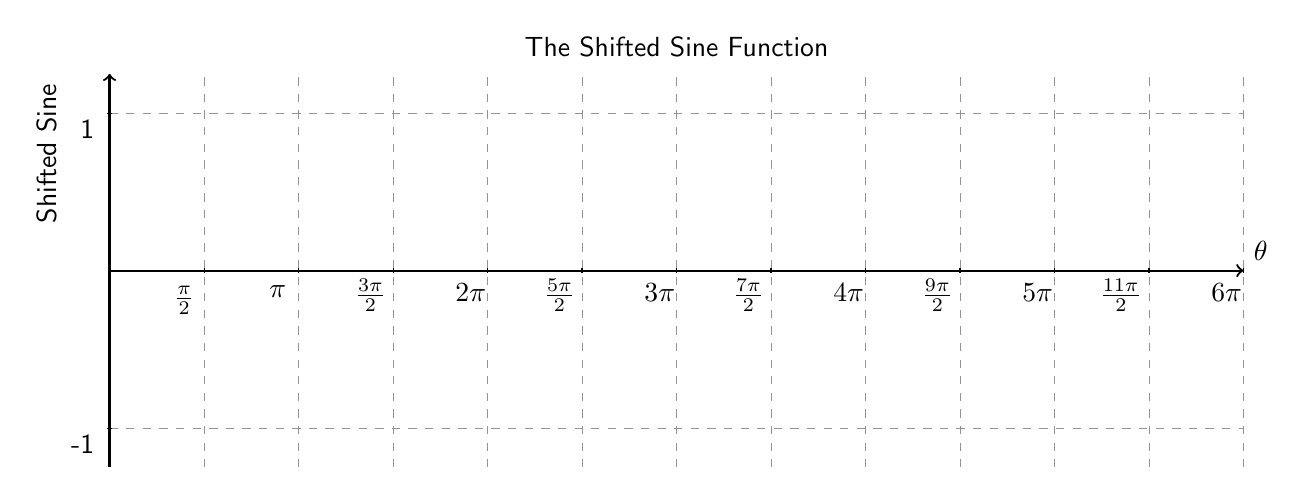
\begin{tikzpicture}[y=2cm, x=1.2cm,font=\sffamily]
      % bounds
      \def\lowX{0.0}
      \pgfmathtruncatemacro\startX{round(0.5+\lowX)}
      \pgfmathsetmacro\nextXValue{int(\startX+1)}
      \def\highX{12}
      \def\lowY{-1.25}
      \def\highY{1.25}
      \pgfmathsetmacro\nextYValue{int(\lowY+1)}
      % ticks
      \draw[step = 1, gray, very thin,dashed,opacity=0.85] (0, \lowY) grid ( \highX,\highY);
      % axis
      \draw[thick,->] (0,0) -- coordinate (x axis mid) (\highX,0) node[anchor = south west] {$\theta$};
      \draw[thick,->] (0,\lowY) -- coordinate (y axis mid) (0,\highY)
           node[rotate=90,yshift=30,anchor = north east] {Shifted Sine};

      \draw (1pt, 1) -- (-1pt, 1) node[yshift=-6,xshift=-1,anchor=east] { 1};
      \draw (1pt,-1) -- (-1pt,-1) node[yshift=-6,xshift=-1,anchor=east] {-1};

      \draw (1,1pt) -- (1,-1pt) node[yshift=-1,xshift=0,anchor=north east] {$\frac{ \pi}{2}$};
      \foreach \x in {3,5,...,\highX} {
        \draw (\x,1pt) -- (\x,-1pt) node[yshift=-8,xshift=1,anchor=east] {$\frac{\x\pi}{2}$};
      }
      \draw (2,1pt) -- (2,-1pt) node[yshift=-1,xshift=-1,anchor=north east] {$\pi$};
      \foreach \x in {2,3,...,6} {
        \draw (2*\x,1pt) -- (2*\x,-1pt) node[yshift=-7,xshift=3,anchor=east] {$\x\pi$};
      }
      \draw (6,1.3) node [anchor=south] {The Shifted Sine Function};
    \end{tikzpicture}

  \clearpage

\item Make a sketch of the cosine function.

  \hspace*{-5em}
  \begin{tikzpicture}[y=2cm, x=1.2cm,font=\sffamily]
      % bounds
      \def\lowX{0.0}
      \pgfmathtruncatemacro\startX{round(0.5+\lowX)}
      \pgfmathsetmacro\nextXValue{int(\startX+1)}
      \def\highX{12}
      \def\lowY{-1.25}
      \def\highY{1.25}
      \pgfmathsetmacro\nextYValue{int(\lowY+1)}
      % ticks
      \draw[step = 1, gray, very thin,dashed,opacity=0.85] (0, \lowY) grid ( \highX,\highY);
      % axis
      \draw[thick,->] (0,0) -- coordinate (x axis mid) (\highX,0) node[anchor = south west] {$\theta$};
      \draw[thick,->] (0,\lowY) -- coordinate (y axis mid) (0,\highY) node[anchor = north east] {Cosine};

      \draw (1pt, 1) -- (-1pt, 1) node[yshift=-6,xshift=-1,anchor=east] { 1};
      \draw (1pt,-1) -- (-1pt,-1) node[yshift=-6,xshift=-1,anchor=east] {-1};

      \draw (1,1pt) -- (1,-1pt) node[yshift=-1,xshift=0,anchor=north east] {$\frac{ \pi}{2}$};
      \foreach \x in {3,5,...,\highX} {
        \draw (\x,1pt) -- (\x,-1pt) node[yshift=-8,xshift=1,anchor=east] {$\frac{\x\pi}{2}$};
      }
      \draw (2,1pt) -- (2,-1pt) node[yshift=-1,xshift=-1,anchor=north east] {$\pi$};
      \foreach \x in {2,3,...,6} {
        \draw (2*\x,1pt) -- (2*\x,-1pt) node[yshift=-7,xshift=3,anchor=east] {$\x\pi$};
      }
      \draw (6,1.3) node [anchor=south] {The Cosine Function};
    \end{tikzpicture}


\item Make a sketch of the cosine function shifted left $\frac{\pi}{2}$ units.

  \hspace*{-5em}
  \begin{tikzpicture}[y=2cm, x=1.2cm,font=\sffamily]
      % bounds
      \def\lowX{0.0}
      \pgfmathtruncatemacro\startX{round(0.5+\lowX)}
      \pgfmathsetmacro\nextXValue{int(\startX+1)}
      \def\highX{12}
      \def\lowY{-1.25}
      \def\highY{1.25}
      \pgfmathsetmacro\nextYValue{int(\lowY+1)}
      % ticks
      \draw[step = 1, gray, very thin,dashed,opacity=0.85] (0, \lowY) grid ( \highX,\highY);
      % axis
      \draw[thick,->] (0,0) -- coordinate (x axis mid) (\highX,0) node[anchor = south west] {$\theta$};
      \draw[thick,->] (0,\lowY) -- coordinate (y axis mid) (0,\highY) node[anchor = north east] {Cosine};

      \draw (1pt, 1) -- (-1pt, 1) node[yshift=-6,xshift=-1,anchor=east] { 1};
      \draw (1pt,-1) -- (-1pt,-1) node[yshift=-6,xshift=-1,anchor=east] {-1};

      \draw (1,1pt) -- (1,-1pt) node[yshift=-1,xshift=0,anchor=north east] {$\frac{ \pi}{2}$};
      \foreach \x in {3,5,...,\highX} {
        \draw (\x,1pt) -- (\x,-1pt) node[yshift=-8,xshift=1,anchor=east] {$\frac{\x\pi}{2}$};
      }
      \draw (2,1pt) -- (2,-1pt) node[yshift=-1,xshift=-1,anchor=north east] {$\pi$};
      \foreach \x in {2,3,...,6} {
        \draw (2*\x,1pt) -- (2*\x,-1pt) node[yshift=-7,xshift=3,anchor=east] {$\x\pi$};
      }
      \draw (6,1.3) node [anchor=south] {The Cosine Function};
    \end{tikzpicture}


\end{problem}


\actTitle{Graphs of Trigonometric Functions}
\begin{problem}
\item A sine function is shifted and scaled as described
  below. Make a sketch of its graph first, and then determine the
  formula for the new function.
  \begin{subproblem}
  \item Make a sketch of a sine function that is shifted left
    $\frac{\pi}{2}$ units, oscillates between 2 and -2, and has a
    period of $2\pi$.

    \hspace*{-3.5em}
    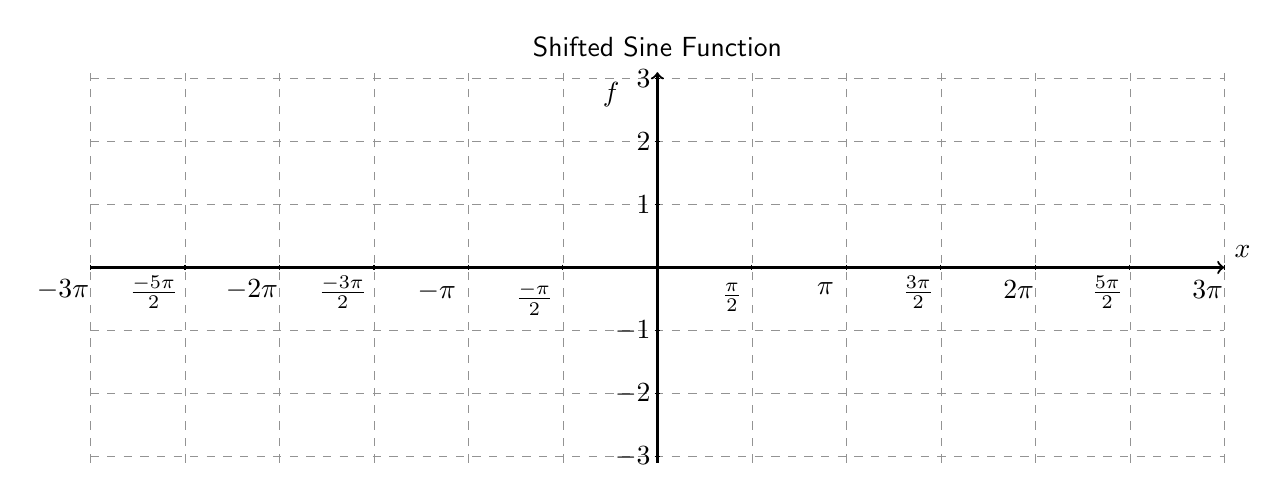
\begin{tikzpicture}[y=0.8cm, x=1.2cm,font=\sffamily]
        % bounds
        \def\lowX{-6}
        \pgfmathtruncatemacro\startX{round(0.5+\lowX)}
        \pgfmathsetmacro\nextXValue{int(\startX+1)}
        \def\highX{6}
        \def\lowY{-3.1}
        \def\highY{3.1}
        \pgfmathsetmacro\nextYValue{int(\lowY+1)}
        % ticks
        \draw[step = 1, gray, very thin,dashed,opacity=0.85] (\lowX, \lowY) grid ( \highX,\highY);
        % axis
        \draw[thick,->] (\lowX,0) -- coordinate (x axis mid) (\highX,0) node[anchor = south west] {$x$};
        \draw[thick,->] (0,\lowY) -- coordinate (y axis mid) (0,\highY) node[xshift=-10,anchor = north east] {$f$};

        \foreach \y in {-3,-2,-1,1,2,3} {
          \draw (-1pt,\y) -- (1pt,\y) node[anchor=east] {$\y$};
        }

        \draw ( 1,1pt) -- ( 1,-1pt) node[yshift=-1,xshift=0,anchor=north east] {$\frac{ \pi}{2}$};
        \draw (-1,1pt) -- (-1,-1pt) node[yshift=-1,xshift=0,anchor=north east] {$\frac{-\pi}{2}$};
        \foreach \x in {-5,-3,3,5} {
          \draw (\x,1pt) -- (\x,-1pt) node[yshift=-8,xshift=1,anchor=east] {$\frac{\x\pi}{2}$};
        }
        \draw ( 2,1pt) -- ( 2,-1pt) node[yshift=-1,xshift=-1,anchor=north east] {$\pi$};
        \draw (-2,1pt) -- (-2,-1pt) node[yshift=-1,xshift=-1,anchor=north east] {$-\pi$};
        \foreach \x in {-3,-2,2,3} {
          \draw (2*\x,1pt) -- (2*\x,-1pt) node[yshift=-7,xshift=3,anchor=east] {$\x\pi$};
        }
        \draw (0,3.2) node [anchor=south] {Shifted Sine Function};
      \end{tikzpicture}


    \item Determine the formula for the new function
      \begin{eqnarray*}
        f(x) & = &
      \end{eqnarray*}
  \end{subproblem}

\item A sine function is shifted and scaled as described
  below. Make a sketch of its graph first, and then determine the
  formula for the new function.
  \begin{subproblem}
  \item Make a sketch of a sine function that is shifted left
    $\frac{\pi}{2}$ units, oscillates between 3 and -1, and has a
    period of $2\pi$.

    \hspace*{-3.5em}
    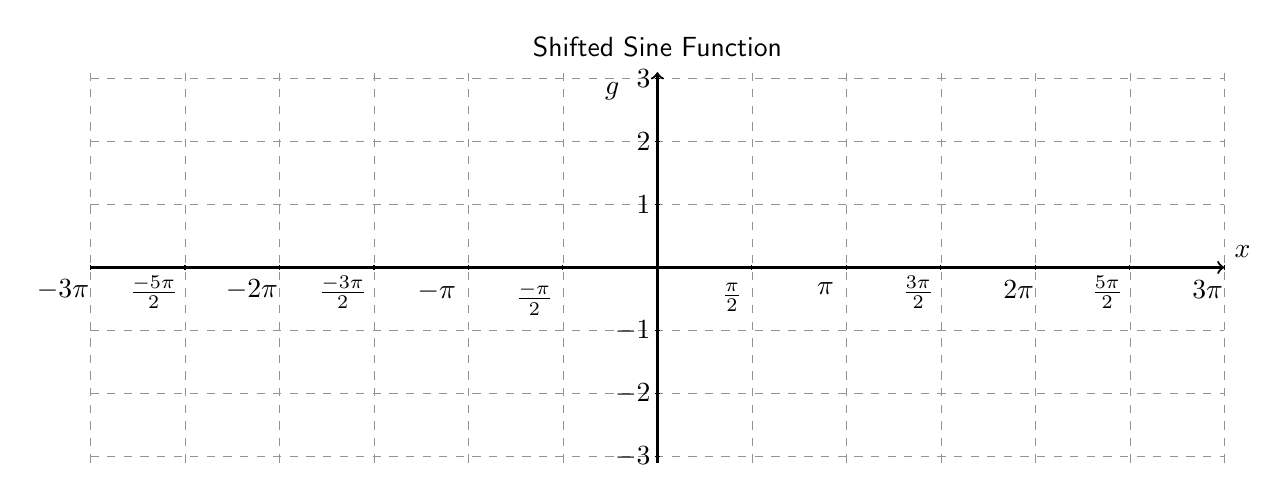
\begin{tikzpicture}[y=0.8cm, x=1.2cm,font=\sffamily]
        % bounds
        \def\lowX{-6}
        \pgfmathtruncatemacro\startX{round(0.5+\lowX)}
        \pgfmathsetmacro\nextXValue{int(\startX+1)}
        \def\highX{6}
        \def\lowY{-3.1}
        \def\highY{3.1}
        \pgfmathsetmacro\nextYValue{int(\lowY+1)}
        % ticks
        \draw[step = 1, gray, very thin,dashed,opacity=0.85] (\lowX, \lowY) grid ( \highX,\highY);
        % axis
        \draw[thick,->] (\lowX,0) -- coordinate (x axis mid) (\highX,0) node[anchor = south west] {$x$};
        \draw[thick,->] (0,\lowY) -- coordinate (y axis mid) (0,\highY) node[xshift=-10,anchor = north east] {$g$};

        \foreach \y in {-3,-2,-1,1,2,3} {
          \draw (-1pt,\y) -- (1pt,\y) node[anchor=east] {$\y$};
        }

        \draw ( 1,1pt) -- ( 1,-1pt) node[yshift=-1,xshift=0,anchor=north east] {$\frac{ \pi}{2}$};
        \draw (-1,1pt) -- (-1,-1pt) node[yshift=-1,xshift=0,anchor=north east] {$\frac{-\pi}{2}$};
        \foreach \x in {-5,-3,3,5} {
          \draw (\x,1pt) -- (\x,-1pt) node[yshift=-8,xshift=1,anchor=east] {$\frac{\x\pi}{2}$};
        }
        \draw ( 2,1pt) -- ( 2,-1pt) node[yshift=-1,xshift=-1,anchor=north east] {$\pi$};
        \draw (-2,1pt) -- (-2,-1pt) node[yshift=-1,xshift=-1,anchor=north east] {$-\pi$};
        \foreach \x in {-3,-2,2,3} {
          \draw (2*\x,1pt) -- (2*\x,-1pt) node[yshift=-7,xshift=3,anchor=east] {$\x\pi$};
        }
        \draw (0,3.2) node [anchor=south] {Shifted Sine Function};
      \end{tikzpicture}


    \item Determine the formula for the new function
      \begin{eqnarray*}
        g(x) & = &
      \end{eqnarray*}
  \end{subproblem}

\clearpage

\item A cosine function is shifted and scaled as described
  below. Make a sketch of its graph first, and then determine the
  formula for the new function.
  \begin{subproblem}
  \item Make a sketch of a cosine function that is shifted right
    $\frac{\pi}{2}$ units, oscillates between 3 and -3, and has a
    period of $2\pi$.

    \hspace*{-3.5em}
    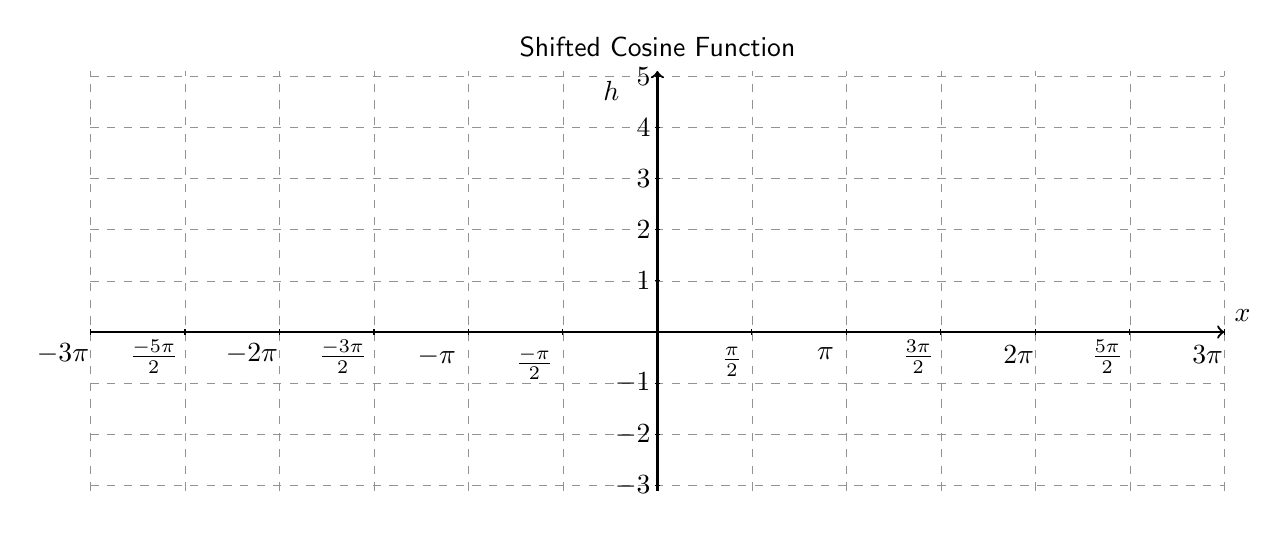
\begin{tikzpicture}[y=0.65cm, x=1.2cm,font=\sffamily]
        % bounds
        \def\lowX{-6}
        \pgfmathtruncatemacro\startX{round(0.5+\lowX)}
        \pgfmathsetmacro\nextXValue{int(\startX+1)}
        \def\highX{6}
        \def\lowY{-3.1}
        \def\highY{5.1}
        \pgfmathsetmacro\nextYValue{int(\lowY+1)}
        % ticks
        \draw[step = 1, gray, very thin,dashed,opacity=0.85] (\lowX, \lowY) grid ( \highX,\highY);
        % axis
        \draw[thick,->] (\lowX,0) -- coordinate (x axis mid) (\highX,0) node[anchor = south west] {$x$};
        \draw[thick,->] (0,\lowY) -- coordinate (y axis mid) (0,\highY) node[xshift=-10,anchor = north east] {$h$};

        \foreach \y in {-3,-2,-1,1,2,...,5} {
          \draw (-1pt,\y) -- (1pt,\y) node[anchor=east] {$\y$};
        }

        \draw ( 1,1pt) -- ( 1,-1pt) node[yshift=-1,xshift=0,anchor=north east] {$\frac{ \pi}{2}$};
        \draw (-1,1pt) -- (-1,-1pt) node[yshift=-1,xshift=0,anchor=north east] {$\frac{-\pi}{2}$};
        \foreach \x in {-5,-3,3,5} {
          \draw (\x,1pt) -- (\x,-1pt) node[yshift=-8,xshift=1,anchor=east] {$\frac{\x\pi}{2}$};
        }
        \draw ( 2,1pt) -- ( 2,-1pt) node[yshift=-1,xshift=-1,anchor=north east] {$\pi$};
        \draw (-2,1pt) -- (-2,-1pt) node[yshift=-1,xshift=-1,anchor=north east] {$-\pi$};
        \foreach \x in {-3,-2,2,3} {
          \draw (2*\x,1pt) -- (2*\x,-1pt) node[yshift=-7,xshift=3,anchor=east] {$\x\pi$};
        }
        \draw (0,5.2) node [anchor=south] {Shifted Cosine Function};
      \end{tikzpicture}


    \item Determine the formula for the new function
      \begin{eqnarray*}
        h(x) & = &
      \end{eqnarray*}
  \end{subproblem}

\item A cosine function is shifted and scaled as described
  below. Make a sketch of its graph first, and then determine the
  formula for the new function.
  \begin{subproblem}
  \item Make a sketch of a cosine function that is shifted right
    $\frac{\pi}{2}$ units, oscillates between 5 and -1, and has a
    period of $2\pi$.

    \hspace*{-3.5em}
    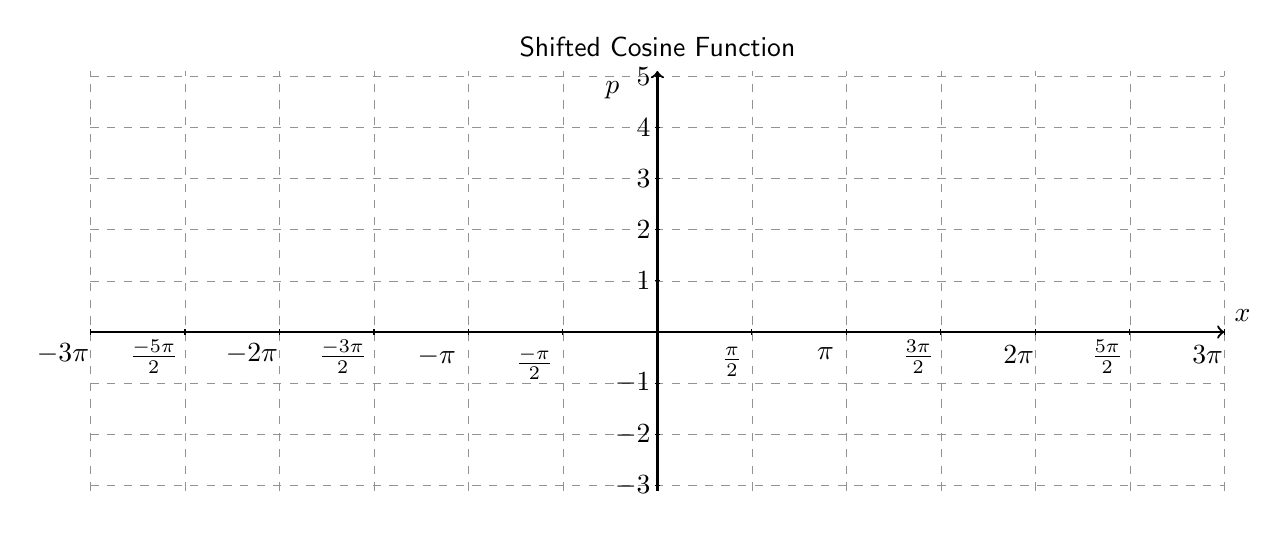
\begin{tikzpicture}[y=0.65cm, x=1.2cm,font=\sffamily]
        % bounds
        \def\lowX{-6}
        \pgfmathtruncatemacro\startX{round(0.5+\lowX)}
        \pgfmathsetmacro\nextXValue{int(\startX+1)}
        \def\highX{6}
        \def\lowY{-3.1}
        \def\highY{5.1}
        \pgfmathsetmacro\nextYValue{int(\lowY+1)}
        % ticks
        \draw[step = 1, gray, very thin,dashed,opacity=0.85] (\lowX, \lowY) grid ( \highX,\highY);
        % axis
        \draw[thick,->] (\lowX,0) -- coordinate (x axis mid) (\highX,0) node[anchor = south west] {$x$};
        \draw[thick,->] (0,\lowY) -- coordinate (y axis mid) (0,\highY) node[xshift=-10,anchor = north east] {$p$};

        \foreach \y in {-3,-2,-1,1,2,...,5} {
          \draw (-1pt,\y) -- (1pt,\y) node[anchor=east] {$\y$};
        }

        \draw ( 1,1pt) -- ( 1,-1pt) node[yshift=-1,xshift=0,anchor=north east] {$\frac{ \pi}{2}$};
        \draw (-1,1pt) -- (-1,-1pt) node[yshift=-1,xshift=0,anchor=north east] {$\frac{-\pi}{2}$};
        \foreach \x in {-5,-3,3,5} {
          \draw (\x,1pt) -- (\x,-1pt) node[yshift=-8,xshift=1,anchor=east] {$\frac{\x\pi}{2}$};
        }
        \draw ( 2,1pt) -- ( 2,-1pt) node[yshift=-1,xshift=-1,anchor=north east] {$\pi$};
        \draw (-2,1pt) -- (-2,-1pt) node[yshift=-1,xshift=-1,anchor=north east] {$-\pi$};
        \foreach \x in {-3,-2,2,3} {
          \draw (2*\x,1pt) -- (2*\x,-1pt) node[yshift=-7,xshift=3,anchor=east] {$\x\pi$};
        }
        \draw (0,5.2) node [anchor=south] {Shifted Cosine Function};
      \end{tikzpicture}


    \item Determine the formula for the new function
      \begin{eqnarray*}
        p(x) & = &
      \end{eqnarray*}
  \end{subproblem}

\clearpage

\item A sine function is scaled as described below. Make a sketch of
  its graph first, and then determine the formula for the new
  function.
  \begin{subproblem}
  \item Make a sketch of a sine function that has a period of 1 and an
    amplitude of 1. The function oscillates between 1 and -1.

    \hspace*{-3.5em}
    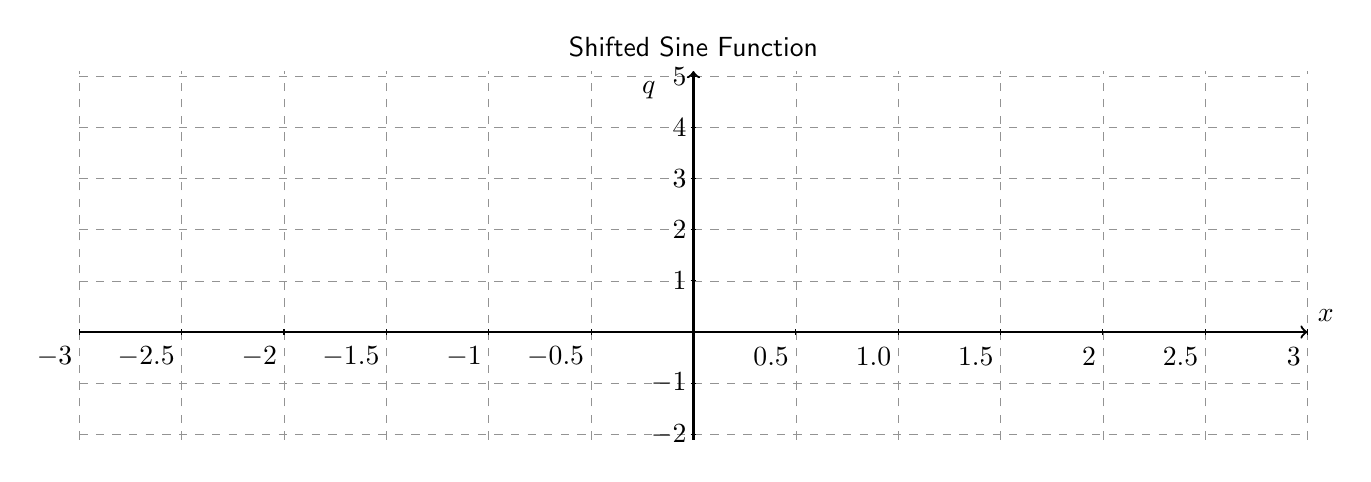
\begin{tikzpicture}[y=0.65cm, x=1.3cm,font=\sffamily]
        % bounds
        \def\lowX{-6}
        \pgfmathtruncatemacro\startX{round(0.5+\lowX)}
        \pgfmathsetmacro\nextXValue{int(\startX+1)}
        \def\highX{6}
        \def\lowY{-2.1}
        \def\highY{5.1}
        \pgfmathsetmacro\nextYValue{int(\lowY+1)}
        % ticks
        \draw[step = 1, gray, very thin,dashed,opacity=0.85] (\lowX, \lowY) grid ( \highX,\highY);
        % axis
        \draw[thick,->] (\lowX,0) -- coordinate (x axis mid) (\highX,0) node[anchor = south west] {$x$};
        \draw[thick,->] (0,\lowY) -- coordinate (y axis mid) (0,\highY) node[xshift=-10,anchor = north east] {$q$};

        \foreach \y in {-2,-1,1,2,...,5} {
          \draw (-1pt,\y) -- (1pt,\y) node[anchor=east] {$\y$};
        }

        \foreach \x in {-3,-2.5,...,-0.5,0.5,1.0,...,3} {
          \draw (2*\x,1pt) -- (2*\x,-1pt) node[yshift=-8,xshift=1,anchor=east] {$\x$};
        }
        \draw (0,5.2) node [anchor=south] {Shifted Sine Function};
      \end{tikzpicture}


  \item Determine the formula for the new function
    \begin{eqnarray*}
        q(x) & = &
    \end{eqnarray*}
  \end{subproblem}

\item A cosine function is shifted and scaled as described
  below. Make a sketch of its graph first, and then determine the
  formula for the new function.
  \begin{subproblem}
  \item Make a sketch of a cosine function that is shifted right
    2 units, oscillates between 5 and -1, and has a period of 1.

    \hspace*{-3.5em}
    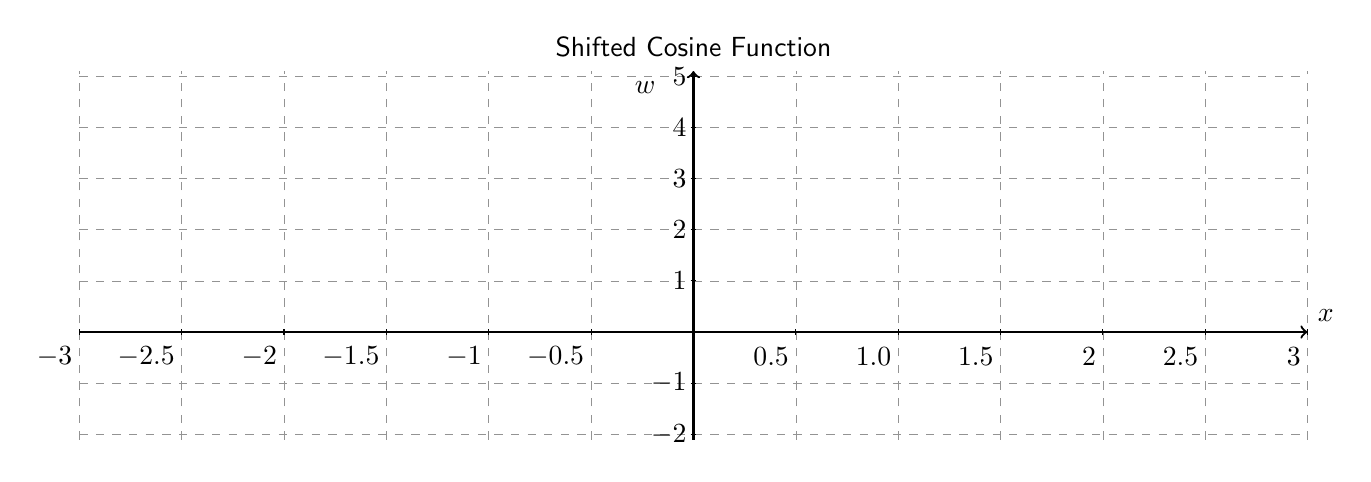
\begin{tikzpicture}[y=0.65cm, x=1.3cm,font=\sffamily]
        % bounds
        \def\lowX{-6}
        \pgfmathtruncatemacro\startX{round(0.5+\lowX)}
        \pgfmathsetmacro\nextXValue{int(\startX+1)}
        \def\highX{6}
        \def\lowY{-2.1}
        \def\highY{5.1}
        \pgfmathsetmacro\nextYValue{int(\lowY+1)}
        % ticks
        \draw[step = 1, gray, very thin,dashed,opacity=0.85] (\lowX, \lowY) grid ( \highX,\highY);
        % axis
        \draw[thick,->] (\lowX,0) -- coordinate (x axis mid) (\highX,0) node[anchor = south west] {$x$};
        \draw[thick,->] (0,\lowY) -- coordinate (y axis mid) (0,\highY) node[xshift=-10,anchor = north east] {$w$};

        \foreach \y in {-2,-1,1,2,...,5} {
          \draw (-1pt,\y) -- (1pt,\y) node[anchor=east] {$\y$};
        }

        \foreach \x in {-3,-2.5,...,-0.5,0.5,1.0,...,3} {
          \draw (2*\x,1pt) -- (2*\x,-1pt) node[yshift=-8,xshift=1,anchor=east] {$\x$};
        }
        \draw (0,5.2) node [anchor=south] {Shifted Cosine Function};
      \end{tikzpicture}

    \item Determine the formula for the new function
      \begin{eqnarray*}
        w(x) & = &
      \end{eqnarray*}
  \end{subproblem}

\clearpage

\item A cosine function is shifted and scaled as described
  below. Make a sketch of its graph first, and then determine the
  formula for the new function.
  \begin{subproblem}
  \item Make a sketch of a cosine function that is shifted right
    1 units, oscillates between 2 and -1, and has a period of 2.

    \hspace*{-3.5em}
    \begin{tikzpicture}[y=0.85cm, x=1.8cm,font=\sffamily]
        % bounds
        \def\lowX{-4}
        \pgfmathtruncatemacro\startX{round(0.5+\lowX)}
        \pgfmathsetmacro\nextXValue{int(\startX+1)}
        \def\highX{4}
        \def\lowY{-2.1}
        \def\highY{3.1}
        \pgfmathsetmacro\nextYValue{int(\lowY+1)}
        % ticks
        \draw[step = 1, gray, very thin,dashed,opacity=0.85] (\lowX, \lowY) grid ( \highX,\highY);
        % axis
        \draw[thick,->] (\lowX,0) -- coordinate (x axis mid) (\highX,0) node[anchor = south west] {$x$};
        \draw[thick,->] (0,\lowY) -- coordinate (y axis mid) (0,\highY) node[xshift=-10,anchor = north east] {$D$};

        \foreach \y in {-2,-1,1,2,...,3} {
          \draw (-1pt,\y) -- (1pt,\y) node[anchor=east] {$\y$};
        }

        \foreach \x in {-4,-3,...,-1,1,2,...,4} {
          \draw (\x,1pt) -- (\x,-1pt) node[yshift=-8,xshift=1,anchor=east] {$\x$};
        }
        \draw (0,3.2) node [anchor=south] {Shifted Cosine Function};
      \end{tikzpicture}


    \item Determine the formula for the new function
      \begin{eqnarray*}
        D(x) & = &
      \end{eqnarray*}
  \end{subproblem}

\item A sine function is shifted and scaled as described
  below. Make a sketch of its graph first, and then determine the
  formula for the new function.
  \begin{subproblem}
  \item Make a sketch of a sine function that is shifted left
    2 units, oscillates between -1 and -4, and has a period of
    $\frac{2}{3}$.

    \hspace*{-3.5em}
    \begin{tikzpicture}[y=0.85cm, x=1.8cm,font=\sffamily]
        % bounds
        \def\lowX{-4}
        \pgfmathtruncatemacro\startX{round(0.5+\lowX)}
        \pgfmathsetmacro\nextXValue{int(\startX+1)}
        \def\highX{4}
        \def\lowY{-5.1}
        \def\highY{1.1}
        \pgfmathsetmacro\nextYValue{int(\lowY+1)}
        % ticks
        \draw[step = 1, gray, very thin,dashed,opacity=0.85] (\lowX, \lowY) grid ( \highX,\highY);
        % axis
        \draw[thick,->] (\lowX,0) -- coordinate (x axis mid) (\highX,0) node[anchor = south west] {$x$};
        \draw[thick,->] (0,\lowY) -- coordinate (y axis mid) (0,\highY) node[xshift=-10,anchor = north east] {$L$};

        \foreach \y in {-5,-4,...,-1,1} {
          \draw (-1pt,\y) -- (1pt,\y) node[anchor=east] {$\y$};
        }

        \foreach \x in {-4,-3,...,-1,1,2,...,4} {
          \draw (\x,1pt) -- (\x,-1pt) node[yshift=-8,xshift=1,anchor=east] {$\x$};
        }
        \draw (0,1.2) node [anchor=south] {Shifted Sine Function};
      \end{tikzpicture}


    \item Determine the formula for the new function
      \begin{eqnarray*}
        L(x) & = &
      \end{eqnarray*}
  \end{subproblem}


\end{problem}

\postClass

\begin{problem}
\item Briefly state two ideas from today's class.
  \begin{itemize}
  \item
  \item
  \end{itemize}
\item
  \begin{subproblem}
    \item
  \end{subproblem}
\end{problem}


%%% Local Variables:
%%% mode: latex
%%% TeX-master: "../labManual"
%%% End:
